\section{Bluetooth}
Characteristics:
\begin{itemize}
    \item it comes from SIG (Special Internet Group) $\rightarrow$ big companies join forces\\
    $\Rightarrow$ aim was having a single protocol
    \item it is a standar de facto since a lot of years
    \item main goal $\rightarrow$ cable substitution
    \item it is done for:
    \begin{itemize}
        \item[$\rightarrow$] cordless headset/speakers/printers \dots (devices)
        \item[$\rightarrow$] synchronization among devices $\Rightarrow$ small file sharing
        \item[$\rightarrow$] file sharing
        \item[$\rightarrow$] IOT
        \item[$\rightarrow$] internet bridge $\rightarrow$ to connect device to AP/directly to internet 
        \item[$\rightarrow$] ad hoc networking $\rightarrow$ more difficult to implement 
    \end{itemize}
\end{itemize}
Down here there is a descritption of main features of Bluetooth
\subsection{Architecture}
\begin{itemize}
    \item it is a layered protocol $\rightarrow$ to cover most application layer use cases
    \item each use case need $\rightarrow$ different protocol involved $\rightarrow$ specific profile
    \item architecture is divided in:
    \begin{itemize}
        \item[$\rightarrow$] Core protocols:
        \begin{itemize}
            \item radio $\rightarrow$ used air interface $\Rightarrow$ frequency
            hopping, TX power \dots
            \item baseband $\rightarrow$ connection establishment in Piconet\\
            $\rightarrow$ packet format, timing, addressing
            \item link manager protocol (LMP) $\rightarrow$ bluetooth setup among
            devices,\\security, authentication, encryption
            \item logical link control and adaptation protocol (L2CAP)\\
            $\rightarrow$ adapts upper-layer protocols with Baseband
            \item Service discovery protocol (SDP) $\rightarrow$ it gives device info/address\\
            + establish connection with multiple bluetooth devices
        \end{itemize} 
        \item[$\rightarrow$] Mid protocols:
        \begin{itemize}
            \item cable replacement protocol $\rightarrow$ RFCOMM $\rightarrow$virtual serial port
            \item telephony control protocol $\rightarrow$ TCS BIN $\rightarrow$ binary
        \end{itemize}
        \item[$\rightarrow$] Adopted protocols $\rightarrow$ use of existing and invent new only if necessary:
        \begin{itemize}
            \item PPP (Point-to-Point (P$_2$P) protocol) $\rightarrow$ IP datagrams are over P$_2$P link
            \item TCP/UDP/IP
            \item OBEX (Object Exchange protocol) $\rightarrow$ it defines object operations
            \item WAE/WAP (Wireless Application Environment/Protocol)
        \end{itemize} 
    \end{itemize}
    \item this structure can lead to:
    \begin{itemize}
        \item[$\rightarrow$] high interoperability
        \item[$\rightarrow$] combination of different protocols $\rightarrow$ different bluetooth models
        \item[$\rightarrow$] possiblity to jump over layers which are far from each other
    \end{itemize}
\end{itemize}

\subsection{Topology}
Before talking about topology, there are some parameters of bluetooth radio and baseband
\begin{itemize}
    \item up to 7 simultaneous links in a logical star
    \item max data rate $=$ 1 Mbps
    \item radio frequency bandwidth $=$ 2.4 GHz $\rightarrow$ changing channels n $=$ 0,\dots,78\\
    adding n MHz to 2.4 GHz $\Rightarrow$ up to 2.4835 GHz
    \item carrier spacing $=$ 1 MHz
    \item access:
    \begin{itemize}
        \item[$\rightarrow$] Piconet: FH-TDD-TDMA
        \item[$\rightarrow$] Scatternet: FH-CDMA
    \end{itemize}
\end{itemize}
There are 3 types of topology:
\begin{itemize}
    \item Piconet:
    \begin{itemize}
        \item[$\rightarrow$] collection of devices connected in an ad-hoc fashion
        \item[$\rightarrow$] basic unit of bluetooth $\rightarrow$ there are two types:
        \begin{itemize}
            \item master
            \item slave
        \end{itemize} 
        \item[$\rightarrow$] One unit will act as master $\Rightarrow$ others as slaves for duration of connection
        \item[$\rightarrow$] Master sets clock and hopping pattern $\rightarrow$ determine channel and phase
        \item[$\rightarrow$] Each piconet has a unique hopping pattern/ID
        \item[$\rightarrow$] Each master can connect to 7 simultaneous slaves or 200+
        inactive\\(parked) slaves per piconet
        \item[$\rightarrow$] Setup and formation:
        \begin{enumerate}
            \item Inquiry scan protocol $\rightarrow$ to learn about:
            \begin{itemize}
                \item the clock offset
                \item device address of other nodes in proximity 
            \end{itemize}
            \item Page scan protocol $\rightarrow$ to establish links with nodes in proximity
        \end{enumerate}
        \newpage
        \item[$\rightarrow$] Communication $\rightarrow$ RR Polling:
        \begin{itemize}
            \item master:
            \begin{itemize}
                \item forwards other slave's messages
                \item asks if it has something to send
            \end{itemize}
            $\Rightarrow$ never messages collision (MAC)
            \item time id divided into slots
            \item longer messages can occupy more slots $\rightarrow$ master choice
        \end{itemize}
    \end{itemize}
    \item Point-to-Point link:
    \begin{itemize}
        \item[$\rightarrow$] it is a master slave relationship only
        \item[$\rightarrow$] nodes can act as masters or slaves
    \end{itemize}
    \item Scatternet:
    \begin{itemize}
        \item[$\rightarrow$] it consists on interconnected piconets
        \item[$\rightarrow$] there is only one master per piconet
        \item[$\rightarrow$] shared node can be for piconet$_1$ / piconet$_2$ :
        \begin{itemize}
            \item slave/slave
            \item slave/master (or viceversa)
            \item node with special features
        \end{itemize}
        $\Rightarrow$ node can't be master of 2 piconets connected simultaneously\\
        $\rightarrow$ no central network structure
        \item[$\rightarrow$] it allows many devices to share same area
        \item[$\rightarrow$] it makes efficient use of bandwidth
    \end{itemize}
\end{itemize}
\subsection{Adressing, Error Correction \& Versions}
\begin{itemize}
    \item Addressing:
    \begin{itemize}
        \item[$\rightarrow$] Bluetooth Device address (BD\_ADDR) $\rightarrow$ 48 bit IEEE MAC address
        \item[$\rightarrow$] Active Member address (AM\_ADDR)\\$\rightarrow$ 3 bits active slave address + all zero broadcast address
        \item[$\rightarrow$] Parked Member address (PM\_ADDR) $\rightarrow$ 8 bit parked slave address
    \end{itemize}
    \item Error Correction:
    \begin{itemize}
        \item[$\rightarrow$] useful for avoiding transmissions (if possible)
        \item[$\rightarrow$] there are different schemas $\rightarrow$ (+/- redundancy, +/- bandwidth)
        \item[$\rightarrow$] so:
        \begin{itemize}
            \item $\frac{1}{3}$ rate FEC\footFEC
            $\rightarrow$ used on 18-bit message header, voice field in HV1
            \item $\frac{2}{3}$ rate FEC $\rightarrow$ used in DM, DV, FHS, HV2 packets
            \item ARQ (Automatic Repeat reQuest) $\rightarrow$ used in both DH/DM packets\\
            $\Rightarrow$ some cases:
            \begin{itemize}
                \item Error detection $\rightarrow$ destination detects errors $\Rightarrow$ packets discarded
                \item Positive ACK $\rightarrow$ destination returns positive ACK
                \item Retransmission after timeout $\rightarrow$ if packet unacknowledged\\
                $\Rightarrow$ source retransmits
                \item Negative acknowledgment and retransmission\\
                $\rightarrow$ destination returns negative ACK for packets with errors\\
                $\Rightarrow$ source retransmits
            \end{itemize}
        \end{itemize}
    \end{itemize}
    \item Versions:
    \begin{itemize}
        \item[$\rightarrow$] Bluetooth 1.0 (1.1, 1.2)
        \item[$\rightarrow$] Bluetooth 2.0 (2.1) $\rightarrow$ up to 3 Mbps and reduced latency
        \item[$\rightarrow$] Bluetooth 3.0 $\rightarrow$ improved speed and cooperation with Wi-Fi
        \item[$\rightarrow$] Bluetooth 4.0
        \begin{itemize}
            \item LE: Low Energy (speed up to 1Mbps)
            \item UWB: Ultra Wideband
        \end{itemize}
        \item[$\rightarrow$] Bluetooth 4.1 $\rightarrow$ improved interaction with 4G LTE
        \item[$\rightarrow$] Bluetooth 4.2 $\rightarrow$ improved interaction with IOT
        \item[$\rightarrow$] Bluetooth 5.0 $\rightarrow$ improved range, speed and interference avoidance
    \end{itemize}
\end{itemize}
\subsection{ZigBee}
Characteristics:
\begin{itemize}
    \item created to satisfy new market needs:
    \begin{itemize}
        \item[$\rightarrow$] no new wires
        \item[$\rightarrow$] easy to install and mantain $\rightarrow$ self-organizing, mesh networking
        \item[$\rightarrow$] reliable $\rightarrow$ mesh redundancy, multiple channels, interface tolerance
        \item[$\rightarrow$] secure (AES 128) and scalable (65k devices)
        \item[$\rightarrow$] low power consumption $\rightarrow$ can sleep most of time on, long battery life
        \item[$\rightarrow$] low cost 
    \end{itemize}
    \item it uses IEEE 802.15.4 standard
    \begin{itemize}
        \item[$\rightarrow$] it is high level communications protocol
        \item[$\rightarrow$] it uses small, ultra low-power radio frequency $\rightarrow$ $\neq$ depending on the region
        \item[$\rightarrow$] low consumption 
    \end{itemize}
    \item target applications:
    \begin{itemize}
        \item[$\rightarrow$] secure networking
        \item[$\rightarrow$] long battery life $\rightarrow$ ok application requiring small amount of bandwidth
        \item[$\rightarrow$] sensor and controls $\rightarrow$ smart home, remote metering, automotive, \dots
    \end{itemize}
    \item it supports 65,536 nodes
    \item basic operations are optimized:
    \begin{itemize}
        \item[$\rightarrow$] time to join network: < 30ms
        \item[$\rightarrow$] from sleeping to active: < 15ms
        \item[$\rightarrow$] channel access time: < 15ms  
    \end{itemize}
    \item it supports mesh networking $\rightarrow$ it guarantees redundancy with multihop
    \item topology can be:
    \begin{itemize}
        \item Mesh
        \item Star
        \item Cluster Tree
    \end{itemize}
    \begin{figure}[!h] 
        \centering 
        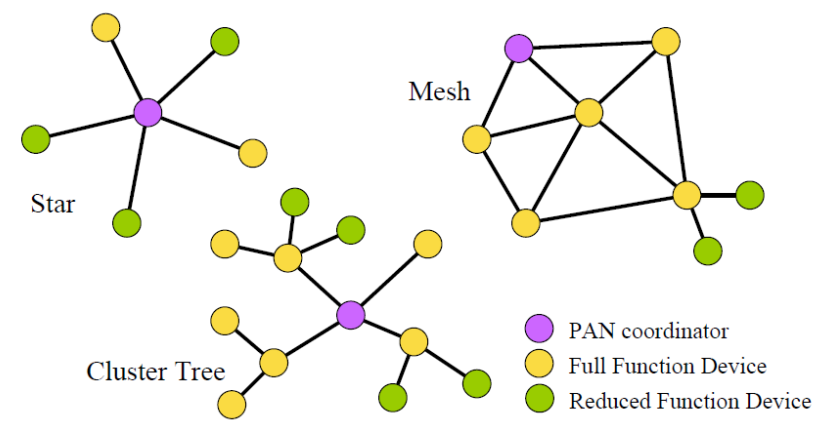
\includegraphics[scale = 0.4]{images/zigbee-topology.png} 
        \caption{Zigbee Topologies}
        \label{zigbee-topology}
    \end{figure}
    \item there are 3 types of nodes:
    \begin{itemize}
        \item[$\rightarrow$] ZigBee Coordinator (ZC):
        \begin{itemize}
            \item each ZB network requires only and only one
            \item it initiates network formation
            \item it may act as router once it is formed
        \end{itemize}
        \newpage
        \item[$\rightarrow$] ZigBee Router (ZR)
        \begin{itemize}
            \item optional network component
            \item it acts as a coordinator
            \item it participates in multihop routing of messages
        \end{itemize}
        \item[$\rightarrow$] ZigBee End Device (ZED)
        \begin{itemize}
            \item optional network component
            \item it shall not allow association or participate in routing
            \item it just send messages
        \end{itemize}  
    \end{itemize}
\end{itemize}

\subsection{ZigBee vs Bluetooth}
Generally:
\begin{itemize}
    \item features $\rightarrow$ each one has its own use case\\
    $\rightarrow$ but ZigBee more suitable for low consumption and low data rate
    \item timing $\rightarrow$ ZigBee faster to perform networking activities + sleep awake trigger
    \item consumption $\rightarrow$ bluetooth more expensive than ZigBee\\
    $\Rightarrow$ but used in mobile phone use case $\rightarrow$ ok
\end{itemize}
The Bluetooth consortium is working on a new version of bluetooth.\\[0.2cm]
Wibree:
\begin{itemize}
    \item performance similar to ZigBee
    \item it is a bluetooth without frequency hopping 
    \item it is a bluetooth with the possibility for nodes
    to be asleep most of the time
    \item it has been adopted into Bluetooth specifications
    \item it will use the same hardware as Bluetooth (shared antenna)
\end{itemize}
\begin{figure}[!h] 
    \centering 
    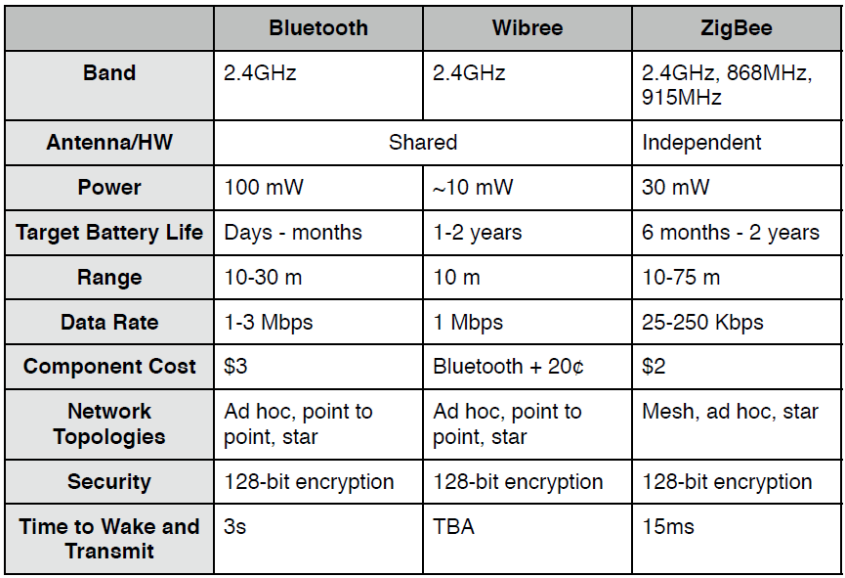
\includegraphics[scale = 0.3]{images/bluetooth-vs-zigbee-vs-wibree.png} 
    \caption{Bluetooth vs Wibree vs Zigbee}
    \label{bluetooth-vs-zigbee-vs-wibree}
\end{figure}